
\documentclass{article}
\usepackage{siunitx} % Provides the \SI{}{} and \si{} command for typesetting SI units
\usepackage{graphicx} % Required for the inclusion of images
\usepackage{natbib} % Required to change bibliography style to APA
\usepackage{amsmath} % Required for some math elements 
\setlength\parindent{24pt} % Removes all indentation from paragraphs
\renewcommand{\labelenumi}{\alph{enumi}.} % Make numbering in the enumerate environment by letter rather than number (e.g. section 6)
\usepackage{times} % Uncomment to use the Times New Roman font
\title{Determination of the Refractive Indexes \\ of Air and Acrylic \\ } % Title
\author{Yi \textsc{Hu}} % Author name
\date{\today} % Date for the report

%----------------------------------------------------------------------------------------
%	%----------------------------------------------------------------------------------------
%	Stitileoage
%----------------------------------------------------------------------------------------
%----------------------------------------------------------------------------------------

\begin{titlepage}
\begin{document}
		\maketitle % Insert the title, author and date
		\thispagestyle{empty}

	
	\begin{center}
		\begin{tabular}{l r}
			Date Performed: & March 2, 2016 \\ % Date the experiment was performed
			Partners: & Yi Hu \\ % Partner names
			& Trina Le \\
			Instructor: & Kyle Slinker % Instructor/supervisor
		\end{tabular}
	\end{center}
\end{titlepage}




%----------------------------------------------------------------------------------------
%	SECTION 1
%----------------------------------------------------------------------------------------

\section{Abstract}


%----------------------------------------------------------------------------------------
%	SECTION 2
%----------------------------------------------------------------------------------------
\section{Theory}
The index of refraction $n$ is the ratio of the speed of light in a vacuum $c$ to the speed of light in a medium $v$. $n=\dfrac{c}{v}$. When light passes through a different medium, it will bend as the wavelength $\lambda$ changes. In this experiment, we used this property of light to measure the refractive indexes of air and acrylic sheet with a Michelson Interferometer for the observation of the interference pattern.

%----------------------------------------------------------------------------------------
%	SECTION 2.1
%----------------------------------------------------------------------------------------
\subsection{Michelson Interferometer}
The Michelson Interferometer is shown next page in Fig.1. When the source light passed through the splitter, half headed toward mirror 1 while the other half was reflected toward mirror 2. When these two beams reflected back by the mirrors, they met and were superimposed, creating a fringe pattern of interference. In the bright regions of the pattern, the crests of the waves of the two beams arrive together. In the dark areas, the crest of one wave arrives at the same time as the trough of the other. 

In this lab, we did not change the physical path length of the beams, but instead changed the optical path length $\tau$. The optical path length of light passing through multiple mediums is equal to $\Sigma n_{i}L_{i}$, where $n_{i}$ is the refractive index of the each individual medium and $L_{i}$ is the physical path length within the medium. If the optical path length of one beam changes by one wavelength, the interference pattern is shifted by one fringe. 
\begin{figure}[htb]
	\begin{center}
		\includegraphics[width=0.40\textwidth]{picture1} % Include the image placeholder.png
		\caption{Michelson Interferometer.}
	\end{center}
\end{figure}

%----------------------------------------------------------------------------------------
%	SECTION 2.2
%----------------------------------------------------------------------------------------
\subsection{Index of Refraction of Air}
To determine the index of refraction of air, we altered the optical path length by placing a vacuum chamber in front of one of the mirrors, as shown in Fig. 2, and pumped out the air slowly until a state of vacuum. In this way, we changed the optical path length of one beam by creating a vacuum environment halfway through, but left that of the other beam unchanged. This resulted in a shift in the observed interference pattern of constructive and destructive interference. 

\begin{figure}[htb]
	\begin{center}
		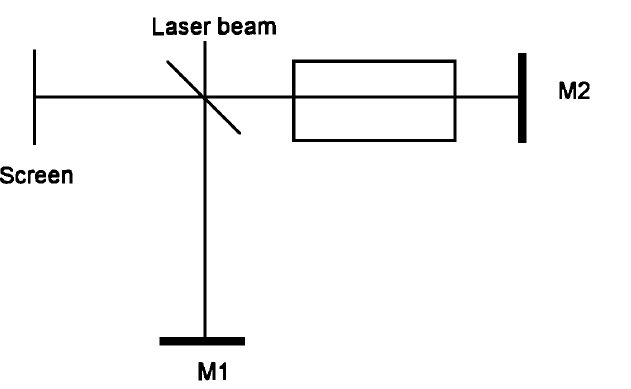
\includegraphics[width=0.65\textwidth]{picture2} % Include the image placeholder.png
		\caption{The setup for determining the refractive index of air.}
	\end{center}
\end{figure}

For air and other ideal gases, the difference between the refractive index and 1 (which is the refractive index of vacuum) is proportional to the pressure of the gas. Thus the index of refraction within the chamber dropped slowly as the pressure decreased, and reached 1 when all the air was pumped out. Suppose the refraction index of air is $n_{air}$, and the air pressure is $p$, then we have
\begin{equation}
	n_{air}=1+kp
\end{equation}

where $k$ is an unknown constant. 

So when the pressure is changed, the corresponding change in the refraction index is
\begin{equation}
\Delta{n}=k\Delta{p}
\end{equation} 

In our experiment, the optical path length within the chamber is $nL$, where $n$ is the refractive index and $L$ is the length of the chamber. Since the beam passed through the chamber twice, and the refractive index changed from that of the air to that of vacuum, we altered the optical path length by $2L\Delta{n}$, in which $\Delta{n}$ is the change in refractive index caused by the change in pressure. 
\begin{equation}
	\Delta{\tau}=2L\Delta{n}
\end{equation}

On the other hand, as the air was being removed, the interference pattern would shift by one fringe at each time the optical path length was changed by one wavelength $\lambda$. So the relation between the observed number of shifts in fringes $m$ and the change in optical path length is 
\begin{equation}
	\Delta{\tau}=m\lambda
\end{equation}

Based on Equ.(2),(3), and(4), we get the unknown constant $k$ to be 
\begin{equation}
	k=\dfrac{m\lambda}{2L\Delta{p}}
\end{equation} 
and if we measured $m$ fringes while the pressure changed by an amount of $\Delta{p}$, we could calculate the refractive index of air at room temperature with
\begin{equation}
	n_{air}=1+\dfrac{m\lambda{p}}{2L\Delta{p}}.
\end{equation}

By plotting $m$ as a function of $\Delta{p}$, we have 
\begin{equation}
	m=\dfrac{2L(n_{air}-1)}{p\lambda}\Delta{p},
\end{equation}
with the slope $k=\dfrac{2L(n_{air}-1)}{p\lambda}$. Thus we can calculate the index of refraction for air to be 
\begin{equation}
	n_{air}=\dfrac{k\lambda{p}}{2L}+1.
\end{equation}

%----------------------------------------------------------------------------------------
%	SECTION 2.3
%----------------------------------------------------------------------------------------
\subsection{Index of Refraction of Acrylic}
To measure the refractive index for acrylic, we replaced the vacuum chamber by a rotation stage that held an acrylic sheet and measured the angle through which it had been turned. Under this setup, we changed the optical path length of one beam by rotating the acrylic sheet. For the same reason that we only changed the path length of one beam, a shift in the interference pattern could be observed and recorded for the calculation of of the refractive index of acrylic. 

Suppose the thickness of the acrylic sheet is $t$ and OP is the original direction of light normal to the sheet, as shown in Fig. 3. Since the refractive index of the air is very close to that of vacuum, we can reasonably assume the index of refraction of air to be 1. Thus the total optical path length between a and c initially for the propagation of light is $nt+bc$ in which $n$ is the index of refraction of acrylic. When acrylic sheet is rotated through an angle $i$, the angles of incidence and refraction are $i$ and $r$ respectively (when the light beam first encounters the acrylic sheet), and the optical path length becomes $ad*n+de$.

\begin{figure}[htb]
	\begin{center}
		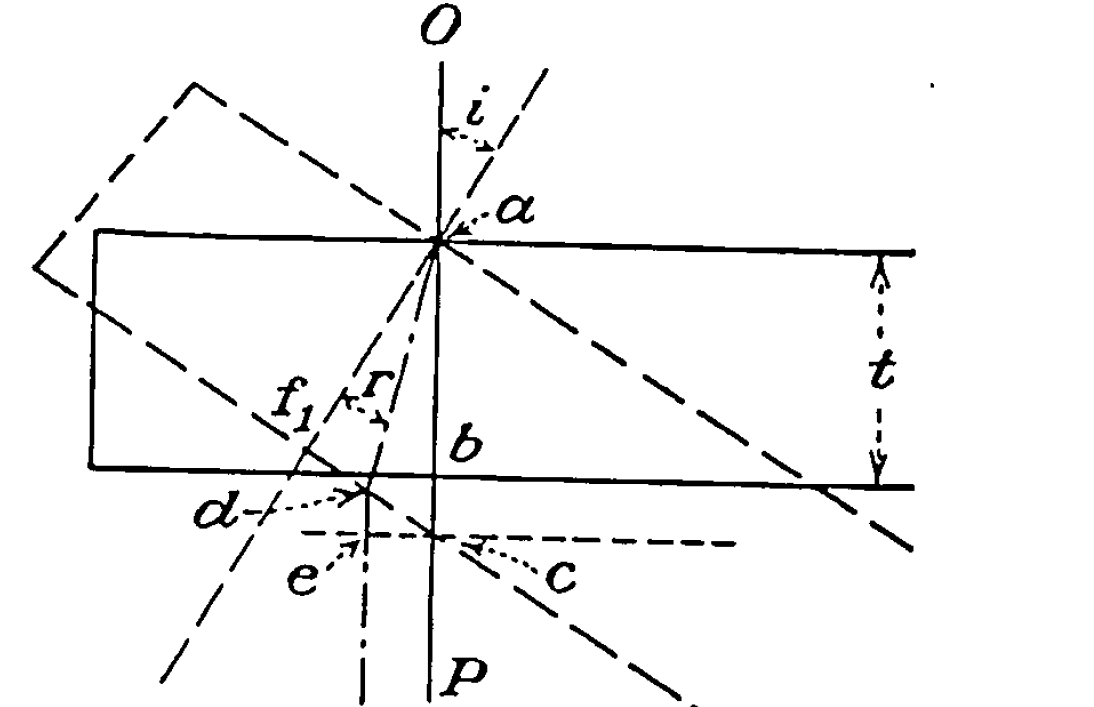
\includegraphics[width=0.5\textwidth]{picture4} % Include the image placeholder.png
		\caption{A light beam travels through an acrylic sheet.}
	\end{center}
\end{figure}

So the change in optical path length equals
\begin{equation}
	\Delta{\tau}=2(n\times{t}+bc-ad\times{n}-de)
\end{equation}
the path length is doubled because the light beam goes through the sheet twice.

Based on the trangles in Fig. 3, we have $ ad=\dfrac{t}{\cos{r}} $, $ bc= \dfrac{t}{\cos{i}}-t$, and $ de=cd\sin{i}=(cf-df)\sin{i}$, in which $cf=t\tan{i}$ and $df=t\tan{r}$. With these relations we get
\begin{equation}
	\Delta{\tau}=2(n{t}+\dfrac{t}{\cos{i}}-t-\dfrac{nt}{\cos{r}}-t\dfrac{sin{i}^{2}}{\cos{i}}+t\tan{r}\sin{i})
\end{equation}



Snell's Law gives
\begin{equation}
	\sin{i}=n\sin{r}
\end{equation}

Combine Equ.(8) and the relation between the observed number of shifts in fringes $m$ and the change in optical path length $\Delta{\tau}=m\lambda$ we get
\begin{equation}
\dfrac{m\lambda}{2t}=n-1+\sec{i}-\tan{i}\sin{i}+\tan{r}\sin{i}
\end{equation}
with Snell's law and the relation $\sin{r}^{2}+\cos{r}^{2}=1$ we substitude all the $r$ with $i$ and get the relation 
\begin{equation}
\dfrac{m\lambda}{2t}=n+\cos{i}-1-\sqrt{n^{2}-\sin{i}^{2}}
\end{equation}

Solving the equation gives us the relation between the refractive index $n$ and the number of fringes
\begin{equation}
	n=\dfrac{(2t+m\lambda)(1-\cos{i})+(\dfrac{m\lambda}{2t})^{2}}{2t(1-\cos{i})+m\lambda}
\end{equation}

Since $\dfrac{m\lambda}{2t}$ is a small number and its square is close to zore, we approximate $n$ to be 
\begin{equation}
n=\dfrac{(2t+m\lambda)(1-\cos{i})}{2t(1-\cos{i})+m\lambda}
\end{equation}

If we keep the angle of incidence small, we can use a Taylor expansion to approximate $\cos{i}$ to be $1-\dfrac{i^{2}}{2}$, thus we have
\begin{equation}
	m\lambda=2ti^{2}\dfrac{n-1}{2n+i^{2}}
\end{equation}
and $i^{2}$ in the denominator is relatively small compared to $2n$ for small angle, so we can further approximate the relation between the number of fringes and the square of incidence angle to be
\begin{equation}
	m=\dfrac{t(n-1)}{\lambda{n}}i^{2}
\end{equation} 

FInally, if we plot $m$ as a function of $i^{2}$, the slope $k$ will be
\begin{equation}
	k=\dfrac{t(n-1)}{n\lambda},
\end{equation}
which means the index of refraction of acrylic $n$ to be 
\begin{equation}
	n=\dfrac{t}{t-k\lambda}.
\end{equation}

%----------------------------------------------------------------------------------------
%	SECTION 3
%----------------------------------------------------------------------------------------
\section{Procedure}
In this lab, we used a Michelson interferometer, a HeNe laser, a vacuum chamber and a acrylic sheet to measure the refractive index of air and acrylic. 
\begin{enumerate}
	\begin{item}
	 to measure the index of refraction of air
	\end{item}
	\begin{item}
		to measure the index of refraction of an acrylic sheet
	\end{item}
\end{enumerate}

For the determination of refraction index of air, we shined the laser at the Michelson interferometer with a vacuum chamber put in the path of one of the interferometer arms, as shown in Fig. 2. For the acrylic, we replaced the vacuum chamber with a acrylic sheet mounted on a rotation stage. 
\subsection{Alignment}
The interferometer must be aligned before both experiment \textit{a} and \textit{b}. We first set up the equipments as shown in Fig. 2. Then we plugged in and turned on the laser. Attention should be paid not looking directly into the laser beam. 

Since we could not look in the interferometer directly when using a laser, we placed a box as a screen and shined the result pattern onto it. A small lens was used to spread the laser beam passing through the interferometer. 

We covered mirror 1 with a sheet of paper. In this way, only the laser beam that headed toward mirror 2 was reflected. We adjusted the location and orientation of the laser until the return beam was very cloes to the exist hole on the face of the laser. Some light from mirror 2 could be observed on the screen. 

Then we uncovered the mirror 1. This led to another set of light seen on the screen. We turned the screws on mirror 1 until the two sets of light superimposed. An interference pattern of concentric fringes was shown on the screen after we had aligned the interferometer properly. 

\subsection{Experiment a: measure the refraction index of air }



%----------------------------------------------------------------------------------------
%	SECTION 4
%----------------------------------------------------------------------------------------
\section{Analysis}



%----------------------------------------------------------------------------------------
%	SECTION 5
%----------------------------------------------------------------------------------------
\section{Discussion}
% If you have more than one objective, uncomment the below:
%\begin{description}
%\item[First Objective] \hfill \\
%Objective 1 text
%\item[Second Objective] \hfill \\
%Objective 2 text
%\end{description}

\subsection{Definitions}
\label{definitions}
\begin{description}
\item[Stoichiometry]
The relationship between the relative quantities of substances taking part in a reaction or forming a compound, typically a ratio of whole integers.
\item[Atomic mass]
The mass of an atom of a chemical element expressed in atomic mass units. It is approximately equivalent to the number of protons and neutrons in the atom (the mass number) or to the average number allowing for the relative abundances of different isotopes. 
\end{description} 
 


\section{Experimental Data}

\begin{tabular}{ll}
Mass of empty crucible & \SI{7.28}{\gram}\\
Mass of crucible and magnesium before heating & \SI{8.59}{\gram}\\
Mass of crucible and magnesium oxide after heating & \SI{9.46}{\gram}\\
Balance used & \#4\\
Magnesium from sample bottle & \#1
\end{tabular}

%----------------------------------------------------------------------------------------
%	SECTION 3
%----------------------------------------------------------------------------------------

\section{Sample Calculation}

\begin{tabular}{ll}
Mass of magnesium metal & = \SI{8.59}{\gram} - \SI{7.28}{\gram}\\
& = \SI{1.31}{\gram}\\
Mass of magnesium oxide & = \SI{9.46}{\gram} - \SI{7.28}{\gram}\\
& = \SI{2.18}{\gram}\\
Mass of oxygen & = \SI{2.18}{\gram} - \SI{1.31}{\gram}\\
& = \SI{0.87}{\gram}
\end{tabular}

Because of this reaction, the required ratiotwo significant figures).





\section{Answers to Definitions}

\begin{enumerate}
\begin{item}
The \emph{atomic weight of an element} is the relative weight of one of its atoms compared to C-12 with a weight of 12.0000000$\ldots$, hydrogen with a weight of 1.008, to oxygen with a weight of 16.00. Atomic weight is also the average weight of all the atoms of that element as they occur in nature.
\end{item}
\begin{item}
The \emph{units of atomic weight} are two-fold, with an identical numerical value. They are g/mole of atoms (or just g/mol) or amu/atom.
\end{item}
\begin{item}
\emph{Percentage discrepancy} between an accepted (literature) value and an experimental value is
\begin{equation*}
\frac{\mathrm{experimental\;result} - \mathrm{accepted\;result}}{\mathrm{accepted\;result}}
\end{equation*}
\end{item}
\end{enumerate}

%----------------------------------------------------------------------------------------
%	BIBLIOGRAPHY
%----------------------------------------------------------------------------------------

\bibliographystyle{apalike}

\bibliography{sample}

%----------------------------------------------------------------------------------------


\end{document}